\documentclass[a4paper, 12pt]{report}
\usepackage{cmap}
\usepackage{amssymb}
\usepackage{amsmath}
\usepackage{graphicx}
\usepackage{amsthm}
\usepackage{upgreek}
\usepackage{setspace}
\usepackage{color}
\usepackage{moreverb}
\usepackage[T2A]{fontenc}
\usepackage[utf8]{inputenc}
\usepackage[normalem]{ulem}
\usepackage{mathtext} % русские буквы в формулах
\usepackage[left=2cm,right=2cm, top=2cm,bottom=2cm,bindingoffset=0cm]{geometry}
\usepackage[english,russian]{babel}
\usepackage[unicode]{hyperref}
\newenvironment{Proof} % имя окружения
{\par\noindent{$\blacklozenge$}} % команды для \begin
{\hfill$\scriptstyle\boxtimes$}
\newcommand{\Rm}{\mathbb{R}}
\newcommand{\Cm}{\mathbb{C}}
\newcommand{\Z}{\mathbb{Z}}
\newcommand{\I}{\mathbb{I}}
\newcommand{\N}{\mathbb{N}}
\newcommand{\rank}{\operatorname{rank}}
\newcommand{\Ra}{\Rightarrow}
\newcommand{\ra}{\rightarrow}
\newcommand{\FI}{\Phi}
\newcommand{\Sp}{\text{Sp}}
\renewcommand{\leq}{\leqslant}
\renewcommand{\geq}{\geqslant}
\renewcommand{\alpha}{\upalpha}
\renewcommand{\beta}{\upbeta}
\renewcommand{\gamma}{\upgamma}
\renewcommand{\delta}{\updelta}
\renewcommand{\varphi}{\upvarphi}
\renewcommand{\phi}{\upvarphi}
\renewcommand{\tau}{\uptau}
\renewcommand{\lambda}{\uplambda}
\renewcommand{\psi}{\uppsi}
\renewcommand{\mu}{\upmu}
\renewcommand{\omega}{\upomega}
\renewcommand{\d}{\partial}
\renewcommand{\xi}{\upxi}
\renewcommand{\epsilon}{\upvarepsilon}
\newcommand{\intx}{\int\limits_{x_0}^x}
\newcommand\Norm[1]{\left\| #1 \right\|}
\newcommand{\sumk}{\sum\limits_{k=0}^\infty}
\newcommand{\sumi}{\sum\limits_{i=0}^\infty}
\newtheorem*{theorem}{Теорема}
\newtheorem*{cor}{Следствие}
\newtheorem*{lem}{Лемма}
\begin{document}
	% Оформление титульного листа
	\begin{titlepage}
		\begin{center}
			\textsc{МИНИСТЕРСТВО ОБРАЗОВАНИЯ РЕСПУБЛИКИ БЕЛАРУСЬ БЕЛОРУССКИЙ ГОСУДАРСТВЕННЫЙ УНИВЕРСИТЕТ
				\\[5mm]
				ФАКУЛЬТЕТ ПРИКЛАДНОЙ МАТЕМАТИКИ И ИНФОРМАТИКИ\\[2mm]
				Кафедра информационных систем управления
			}
			
			\vfill
			
			\textbf{Отчет по лабораторной работе №4\\
				Вариант 22
				\\[26mm]
			}
		\end{center}
		
		\hfill
		\begin{minipage}{.5\textwidth}
			\begin{flushright}
				Бовта Тимофея Анатольевича\\
				студента 3 курса\\
				специальности «прикладная математика»\\[5mm]
				
				Преподаватель:\\[2mm] 
				Д. Ю. Кваша\\
			\end{flushright}
		\end{minipage}%
		\vfill
		\begin{center}
			Минск, 2024\ г.
		\end{center}
	\end{titlepage}
	\newpage
	\section*{Лабораторная работа №4}
	\subsection*{Постановка задачи.}
	Задача о рюкзаке (англ. Knapsack problem) — дано $n$ предметов, предмет $i$ имеет массу
	$w_i > 0$ и стоимость $p_i > 0$. Необходимо выбрать из этих предметов такой набор, чтобы суммарная масса не превосходила заданной величины W (вместимость рюкзака), а суммарная
	стоимость была максимальна.\\\\
	Рассмотрим задачу \textbf{Неограниченный рюкзак} (англ. Unbounded Knapsack Problem), в
	которой любой предмет может быть выбран любое количество раз.\\\\
	\textbf{Формулировка Задачи}\\
	Каждый предмет может быть выбран любое число раз. Задача выбрать количество $x_i$
	предметов каждого типа так, чтобы
	максимизировать общую стоимость: $$\sum_{i=1}^n p_ix_i,$$
	выполнялось условие совместности: $$\sum_{i=1}^n w_ix_i \leq W;$$
	где $x_i \geq 0$ целое, для всех $i = 1, 2, \ldots , n.$
	\subsection*{Условие задачи.}
	$$\max 4x_1 + 8x_2 + 15x_3 ;$$
	$$s.t.\ 3x_1 + 4x_2 + 5x_3 \leq 10;$$
	$$x_1,x_2,x_3 \in \mathbb Z_+$$
	\subsection*{Программная реализация алгоритма.}
	\listinginput[1]{1}{knapsack.py}
	\subsection*{Результат выполнения программы.}
	$$
		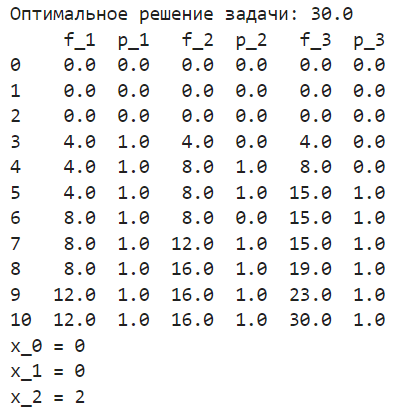
\includegraphics[scale=0.8]{screenshot001}
	$$
	
\end{document}